\section{Discussion}\label{sec:discussion}
\subsection{Traveling standing waves at normal incidence}

Change the absorbing boundary in the second medium to a perfect electric boundary.

\paragraph{Task 2a} \textit{Identify the standing and traveling wave in the structure.}
\begin{figure}[tbph]
	\centering
	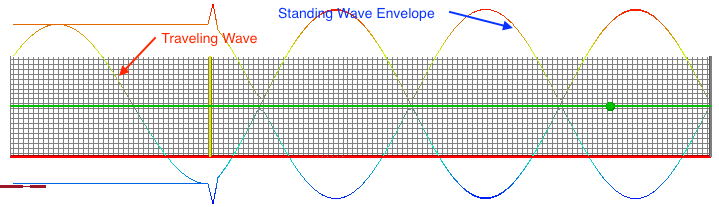
\includegraphics[width=0.95\linewidth]{graphics/Task2-2a-Standing-better-envelope}
	\caption{Standing wave pattern for waveguide with electric boundary at right end}
	\label{fig:Task2-2a-Standing-better-envelope}
\end{figure}

\paragraph{Task 2b} \textit{What is the amplitude of the wave at the probe? Is it \SI{2}{\volt\per\meter}? Why?}
\begin{figure}[tbph]
	\centering
	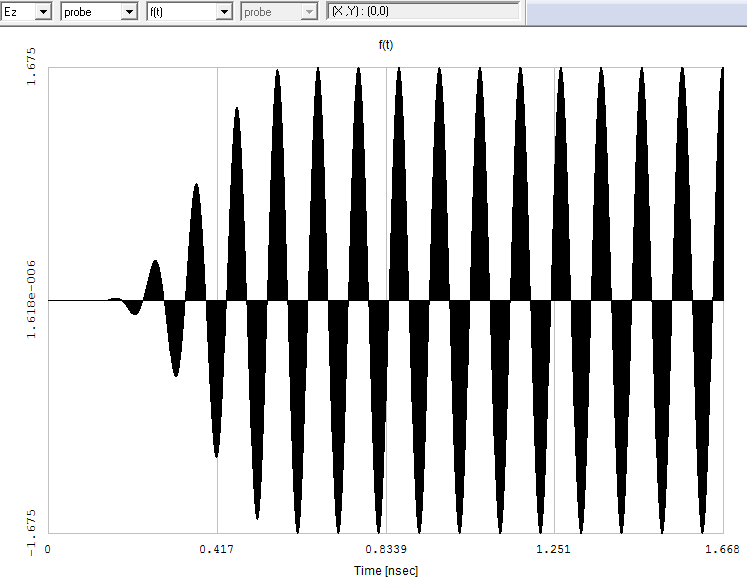
\includegraphics[width=0.6\linewidth]{graphics/Task2-2b-Amplitude}
\end{figure}

The amplitude of the standing wave is \SI{1.675}{\volt\per\meter} because the probe is not located at a standing wave antinode: odd integer multiples of $l_{max}$.

\paragraph{Task 2c} \textit{What is the amplitude of the wave to the left of the source region? Is it \SI{2}{\volt\per\meter}? Why?}

Fig.~\ref{fig:Task2-2a-Standing-better-envelope} shows that the wave has an amplitude of \SI{2}{\volt\per\meter}.
This is because the reflected wave is in phase with the source wave and constructive interference occurs.

\paragraph{Task 2d} \textit{What are: $E_{max}, E_{min}, l_{max}, l_{min}, \left|\Gamma\right|, \phi_\Gamma$? What are possible sources of error between the simulation and expected values?}
\begin{table}[htpb]
	\centering
	\begin{tabular}{@{}ccc@{}}
		\toprule
		Parameter             & Expected                & Actual \\ 
		\midrule
		$E_{max}$             & \SI{2}{\volt\per\meter} & \SI{1.969}{\volt\per\meter} \\
		$E_{min}$             & \SI{0}{\volt\per\meter} & \SI{0.3478}{\volt\per\meter} \\
		$l_{max}$             & \SI{62.5}{\milli\meter} & $<62.5$\si{\milli\meter} \\
		$l_{min}$             & \SI{55}{\milli\meter}   & $<55$\si{\milli\meter} \\
		$\left|\Gamma\right|$ & \sfrac{1}{3}            & \sfrac{1}{3} \\
		$\phi_\Gamma$         & $-\pi$~\si{\radian}     & $-\pi$~\si{\radian} \\ 
		\bottomrule
	\end{tabular}
\end{table}

The values of $E$ differ from the expected values because the probes for those measurements were placed at the positions of $l_{max}$ and $l_{min}$ as determined by calculating the wavelength for $c_0 = \SI{3.0E8}{\meter\per\second}$.

\pagebreak
\paragraph{Task 5a} \textit{Set $\epsilon_{r2} = 4$, $\sigma_2 = \SI{1}{\siemens\per\meter}$ and repeat Task 2 with an absorbing right boundary.}
\begin{figure}[tbph]
	\centering
	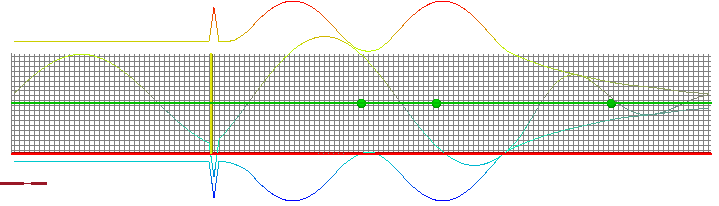
\includegraphics[width=0.95\linewidth]{graphics/Task2-5a-Standing}
	\caption{$\epsilon_{r2} = 4$, $\sigma_2 = \SI{1}{\siemens\per\meter}$, absorbing right boundary}
	\label{fig:Task2-5a-Standing}
\end{figure}

A standing wave envelope is produced between the source and dielectric boundary.
As the wave enters the second medium it is attenuated.

\paragraph{Task 5b} \textit{What is the amplitude of the wave at the probe? Is it \SI{2}{\volt\per\meter}? Why?}
\begin{figure}[tbph]
	\centering
	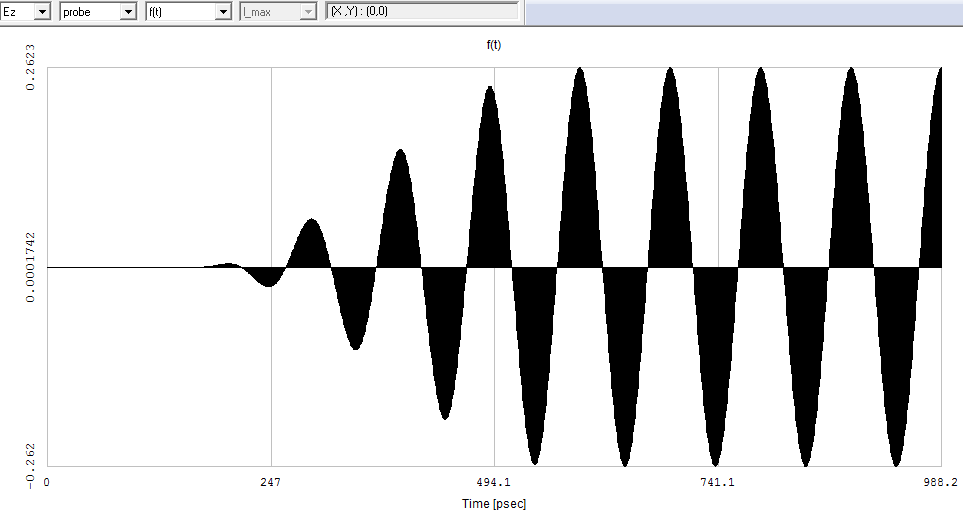
\includegraphics[width=0.6\linewidth]{graphics/Task2-5b-Amplitude}
\end{figure}

The amplitude is \SI{0.263}{\volt\per\meter}.
As noted in 2b, the source is not placed at an antinode.
Also, the wave attenuates as it enters the second medium because $\sigma_2 \ne 0$.

\paragraph{Task 5c} \textit{What is the amplitude of the wave to the left of the source region? Is it \SI{2}{\volt\per\meter}? Why?}
\begin{figure}[tbph]
	\centering
	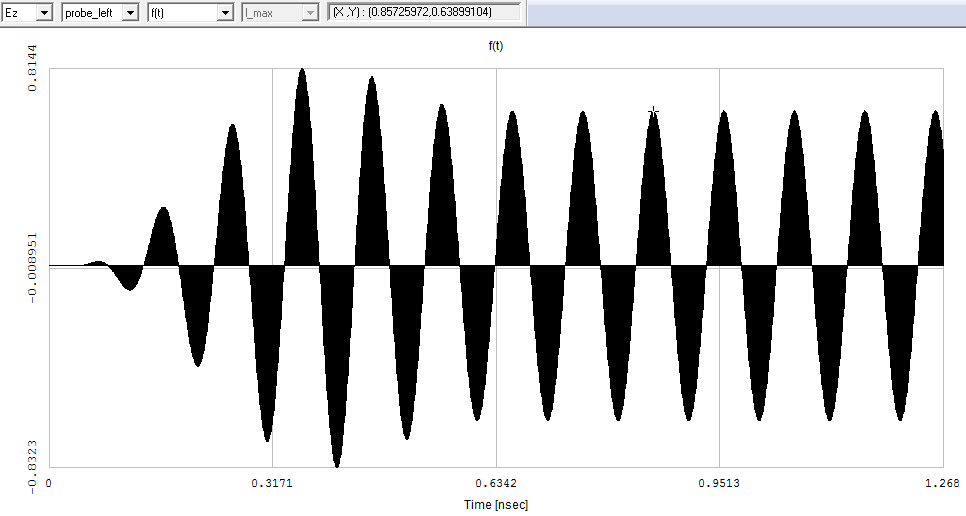
\includegraphics[width=0.6\linewidth]{graphics/Task2-5c-Amplitude_left}
\end{figure}
The amplitude is \SI{0.639}{\volt\per\meter} \textit{I think this value is wrong.
Reading the (x,y) pair in the top of the graph it's the same for all graphs...}

\paragraph{Task 5d} \textit{What are: $E_{max}, E_{min}, l_{max}, l_{min}, \left|\Gamma\right|, \phi_\Gamma$? What are possible sources of error between the simulation and expected values?}
\begin{table}[htpb]
	\centering
	\begin{tabular}{@{}ccc@{}}
		\toprule
		Parameter             & Expected                   & Actual \\ 
		\midrule
		$E_{max}$             & \SI{1.33}{\volt\per\meter} & \SI{1.365}{\volt\per\meter} \\
		$E_{min}$             & \SI{0.67}{\volt\per\meter} & \SI{0.685}{\volt\per\meter} \\
		$l_{max}$             & \SI{42.5}{\milli\meter}    & $>42.5$\si{\milli\meter} \\
		$l_{min}$             & \SI{50}{\milli\meter}      & $>50$\si{\milli\meter} \\
		$\left|\Gamma\right|$ & \sfrac{1}{7}               & \sfrac{1}{7} \\
		$\phi_\Gamma$         & 0~\si{\radian}             & 0~\si{\radian} \\ 
		\bottomrule
	\end{tabular}
\end{table}

Again, error comes from approximating $c_0$.

\paragraph{Task 6a} \textit{Set $\epsilon_{r1} = 9$, $\sigma_1 = \SI{0.5}{\siemens\per\meter}$ and repeat Task 5.}
\begin{figure}[tbph]
	\centering
	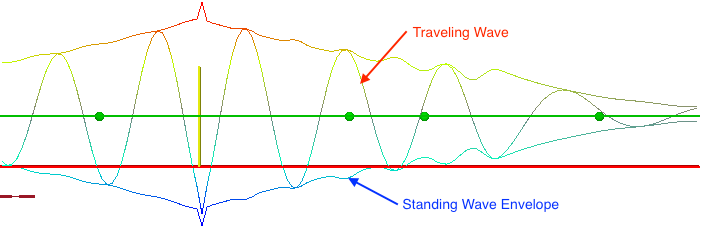
\includegraphics[width=0.96\linewidth]{graphics/Task2-6a-Standing}
	\caption{$\epsilon_{r1} = 9$, $\sigma_1 = \SI{0.5}{\siemens\per\meter}$, $\epsilon_{r2} = 4$, $\sigma_2 = \SI{1}{\siemens\per\meter}$}
	\label{fig:Task2-6a-Standing}
\end{figure}

The wave attenuates in the first dielectric because $\sigma_1 \ne 0$.

\pagebreak
\paragraph{Task 6b} \textit{What is the amplitude of the wave at the probe? Is it \SI{2}{\volt\per\meter}? Why?}
\begin{figure}[tbph]
	\centering
	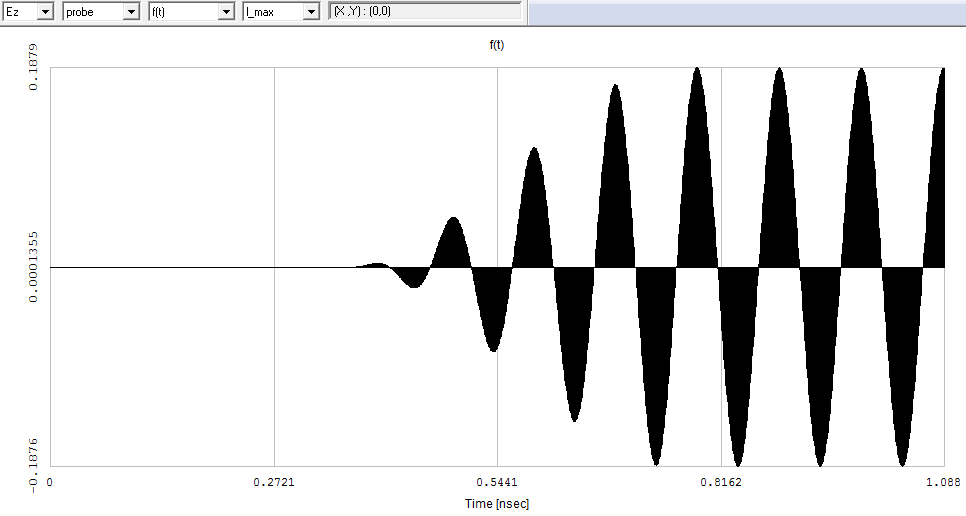
\includegraphics[width=0.6\linewidth]{graphics/Task2-6b-Amplitude}
\end{figure}

The amplitude is \SI{0.1879}{\volt\per\meter}.
It is smaller than in 5b because the wave attenuated in the first medium.

\paragraph{Task 6c} \textit{What is the amplitude of the wave to the left of the source region? Is it \SI{2}{\volt\per\meter}? Why?}
\begin{figure}[tbph]
	\centering
	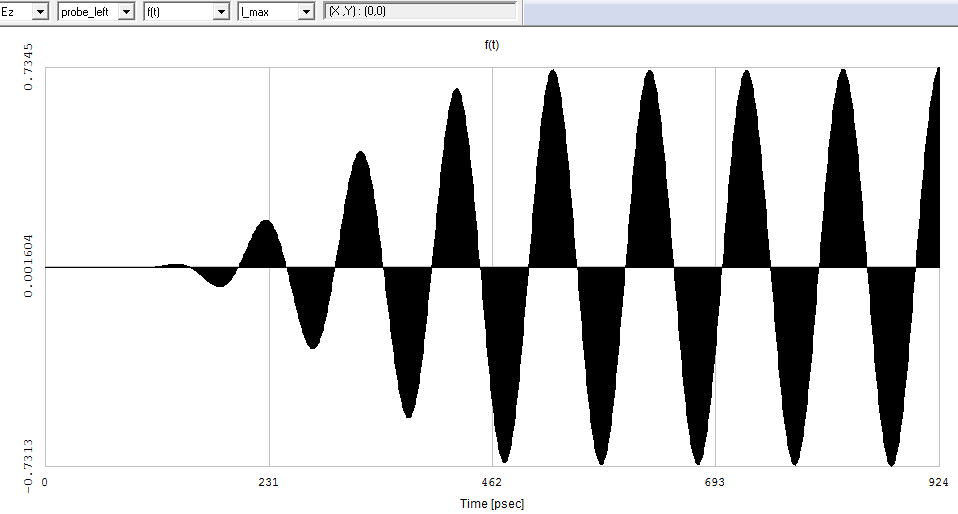
\includegraphics[width=0.6\linewidth]{graphics/Task2-6c-Amplitude_left}
\end{figure}
The amplitude is \SI{0.7345}{\volt\per\meter} at the location of the leftmost probe in Fig.~\ref{fig:Task2-6a-Standing}.
It does not receive constructive interference from the reflection and is attenuated by the dielectric.

\paragraph{Task 6d} \textit{What are: $E_{max}, E_{min}, l_{max}, l_{min}, \left|\Gamma\right|, \phi_\Gamma$? What are possible sources of error between the simulation and expected values?}
\begin{table}[htpb]
	\centering
	\begin{tabular}{@{}ccc@{}}
		\toprule
		Parameter             & Expected                   & Actual \\ 
		\midrule
		$E_{max}$             & ?? & \SI{0.6587}{\volt\per\meter} \\
		$E_{min}$             & ?? & \SI{0.4573}{\volt\per\meter} \\
		$l_{max}$             & \SI{42.5}{\milli\meter}    & $>42.5$\si{\milli\meter} \\
		$l_{min}$             & \SI{50}{\milli\meter}      & $>50$\si{\milli\meter} \\
		$\left|\Gamma\right|$ & ?? & ?? \\
		$\phi_\Gamma$         & ?? & ?? \\
		\bottomrule
	\end{tabular}
\end{table}
